\documentclass[epj]{svjour}

\usepackage{amsmath,amssymb,amsfonts}
\usepackage{physics}
\usepackage{graphicx}
\usepackage{microtype}
\usepackage{tikz}
\usepackage{xparse}
\usepackage{pgfplots}
\pgfplotsset{compat=1.18}

\begin{document}

  \title{Bounded Relational Dynamics and the Structural Necessity of Born--Infeld Geometry}

  \author{J.~Beau}

  \institute{Independent Researcher}

  \date{Received: date / Revised version: date}

  \abstract{
    We investigate how spacetime geometry and non-linear field dynamics can arise as
    equilibrium descriptions of relational systems subject to a finite maximal relaxation flux.
    We show that the existence of a universal bound on admissible relational gradients
    excludes purely quadratic effective actions and uniquely enforces a Born--Infeld-type
    structure as the minimal local representation compatible with saturation.
    Starting from a weighted relational Laplacian with irreversible relaxation,
    we derive an effective continuum description in which the metric tensor emerges
    from the principal symbol of the operator, while antisymmetric perturbations
    enter as an effective gauge field strength.
    In homogeneous regimes, the bounded-relaxation constraint dynamically selects
    flat spacetime with pseudo-Riemannian signature $(-+++)$ as a stable equilibrium.
    When homogeneity is broken by a localized stationary obstruction,
    the same mechanism yields the Schwarzschild geometry as the universal effective exterior solution.
    Horizon formation corresponds to saturation of admissible relational flux and to
    a loss of projectability of the continuum description rather than to a physical singularity.
    These results provide an operator-based unification of Lorentzian geometry,
    Born--Infeld electrodynamics, and horizon formation as consequences of bounded relational dynamics.
  }
%
  \PACS{
      {04.20.-q}{Classical general relativity} \and
    {11.10.Lm}{Nonlinear or nonlocal theories and models} \and
    {03.50.Kk}{Field theories in dimensions other than four}
  }

  \maketitle

  \section{Introduction}
    \label{sec:introduction}

    A growing body of work explores the possibility that spacetime geometry is not a
    fundamental structure but an effective description emerging from more primitive
    relational or operator-based systems.
    In several approaches, discrete relational data, weighted graphs, or spectral operators
    are shown to admit continuum limits in which geometric notions such as distance,
    dimension, and curvature arise as derived quantities rather than postulated ones.
    In particular, it has been demonstrated that, under mild regularity and density
    assumptions, the continuum limit of a relational Laplacian converges to a second-order
    elliptic operator whose principal symbol defines an effective metric tensor~\cite{Beau2026a}.

    While such results establish that effective spacetime geometry can emerge from
    non-geometric relational structures, they leave open a central question:
    why are only very specific geometries observed?
    From a purely mathematical perspective, a large class of elliptic operators and
    corresponding metrics are admissible.
    However, not all such operators necessarily correspond to physically meaningful or
    operationally accessible descriptions.
    Recent analyses have emphasized that effective geometric descriptions may fail when
    the underlying relational structure admits non-injective or degenerate projections,
    leading to a loss of observable factorization and to intrinsic limits of spacetime
    representability~\cite{Beau2026b}.

    This work addresses a complementary and more restrictive problem.
    Rather than asking how geometry can emerge, we ask which effective geometries are
    \emph{dynamically admissible} once minimal physical constraints are imposed on the
    underlying relational dynamics.
    Specifically, we consider relational systems whose effective continuum descriptions
    admit a finite maximal propagation or relaxation speed.
    Such a bound is required for causal consistency and excludes purely quadratic actions,
    which allow arbitrarily large gradients and unbounded fluxes.

    We show that imposing bounded flux propagation uniquely constrains the form of any
    local effective functional governing the continuum limit.
    Under mild assumptions of locality, smoothness, and absence of additional microscopic
    scales, the resulting effective description must take a Born--Infeld--type form.
    This structure is not introduced as a phenomenological modification, but arises as the
    minimal representation compatible with flux saturation.

    Building on this result, we demonstrate that flux saturation does more than regularize
    the effective theory.
    It dynamically selects a restricted class of admissible relational Laplacians whose
    continuum limits define stable and physically meaningful metrics.
    In homogeneous regimes, this selection leads uniquely to flat spacetime.
    In the presence of a localized and stationary obstruction, the same mechanism yields
    the Schwarzschild geometry as the universal effective solution, without postulating
    any independent metric dynamics or field equations.

    Within this framework, horizons are interpreted as loci where flux saturation renders
    the effective operator degenerate, signaling a loss of projectability rather than a
    physical singularity.
    This interpretation aligns naturally with structural analyses of non-injective
    projections and clarifies the operational meaning of strong-field regimes.

    The paper is organized as follows.
    In Section~\ref{sec:bounded-relaxation-and-effective-action}, we establish the necessity of a Born--Infeld--type
    structure from bounded flux propagation.
    Section~\ref{sec:rel-graph-laplacian-op-and-relaxation-dynamics} recalls the emergence of effective
    continuum operators from relational Laplacians.
    Section~\ref{sec:continuum-limit-and-effective-operators} discusses metric reconstruction from operator symbols.
    Sections~\ref{sec:emergence-of-minkowski-spacetime} and~\ref{sec:localized-obstruction-and-schwarzschild-geometry}
    derive flat and Schwarzschild geometries as dynamically selected solutions.
    Section~\ref{sec:horizon-as-flux-saturation-and-loss-of-projectability} analyzes horizon formation as operator
    saturation.
    We conclude with a discussion of scope and limitations.

  \section{Bounded relaxation and effective action}
    \label{sec:bounded-relaxation-and-effective-action}

    We consider effective continuum descriptions arising from relational systems whose
    microscopic dynamics admits a finite maximal propagation or relaxation flux.
    Such a bound is a minimal physical requirement for causal consistency: no influence,
    constraint, or excitation can propagate arbitrarily fast in the effective theory.

    In a continuum regime, the dynamics of slowly varying configurations can be encoded
    in a local action functional
    \begin{equation}
      S = \int d^4x\,\mathcal{L},
    \end{equation}
    where $\mathcal{L}$ depends on the effective fields and their first derivatives.
    From the perspective of field theory, the central question is therefore the following:
    which local Lagrangian densities are compatible with bounded propagation?

    A purely quadratic action, such as the Maxwell form
    \begin{equation}
      \mathcal{L}_{\mathrm{quad}} \propto F_{\mu\nu}F^{\mu\nu},
    \end{equation}
    admits arbitrarily large field gradients.
    As a result, the associated fluxes and characteristic propagation scales are unbounded.
    This behavior is incompatible with the existence of a finite maximal relaxation or
    transport capacity at the microscopic level.

    Imposing bounded propagation requires the effective Lagrangian density to satisfy
    three minimal conditions:
    (i) it reduces to a quadratic form in the weak-field limit,
    (ii) it enforces a strict upper bound on admissible field invariants,
    and (iii) it introduces no additional microscopic scales beyond the saturation scale
    itself.
    Polynomial extensions of quadratic actions fail to meet these requirements without
    fine tuning or the introduction of auxiliary parameters.

    Under these assumptions, the effective Lagrangian density is uniquely constrained to
    take a Born--Infeld--type form.
    Anticipating the operator derivation developed in the following sections, the resulting
    effective action can be written as
    \begin{equation}
      S_{\mathrm{eff}}
      = \beta^2 \int d^4x
      \left(
        \sqrt{-\det\!\left(g_{\mu\nu} + \frac{1}{\beta} F_{\mu\nu}\right)}
        - \sqrt{-\det(g_{\mu\nu})}
      \right),
      \label{eq:BI-action}
    \end{equation}
    where $g_{\mu\nu}$ is the effective metric and $F_{\mu\nu}$ an antisymmetric field strength.
    The parameter $\beta$ sets the maximal admissible field magnitude and fixes the
    saturation scale of the theory.

    The saturation scale $\beta$ will be referred to as the bounded-flux (Born--Infeld)
    scale: it characterizes the maximal admissible relational flux within the validity
    domain of the continuum description.

    In the weak-field regime $|F_{\mu\nu}| \ll \beta$, the expansion of
    Eq.~\eqref{eq:BI-action} yields
    \begin{equation}
      \mathcal{L}_{\mathrm{eff}}
      = -\frac{1}{4}F_{\mu\nu}F^{\mu\nu}
      + \mathcal{O}\!\left(\beta^{-2}\right),\label{eq:equation-weak-field}
    \end{equation}
    showing that standard Maxwell electrodynamics is recovered universally as the
    low-flux approximation of bounded relaxation.
    Non-linear corrections become relevant only when the microscopic saturation scale
    is probed.

    Crucially, the Born--Infeld structure is not introduced here as a phenomenological
    modification of electrodynamics.
    It arises as the minimal local representation compatible with bounded propagation.
    This observation can be formulated as a no-go statement: any local effective action
    admitting a finite maximal flux cannot be purely quadratic in field gradients.
    Born--Infeld electrodynamics therefore represents the unique natural completion of
    Maxwell theory under bounded relaxation.

    \begin{figure}[t]
      \centering
      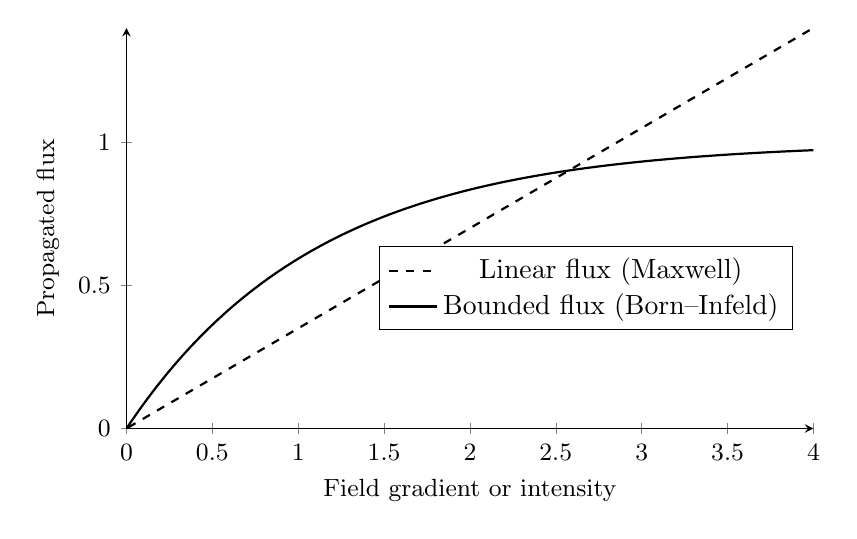
\begin{tikzpicture}
        \begin{axis}[
          width=0.85\columnwidth,
          height=0.55\columnwidth,
          xlabel={Field gradient or intensity},
          ylabel={Propagated flux},
          xmin=0, xmax=4,
          ymin=0, ymax=1.4,
          samples=200,
          axis lines=left,
          legend style={at={(0.97,0.35)},anchor=east},
          ticklabel style={font=\small},
          label style={font=\small}
        ]

          \addplot[thick, dashed]
          {0.35*x};
          \addlegendentry{Linear flux (Maxwell)}

          \addplot[thick]
          {1 - exp(-0.9*x)};
          \addlegendentry{Bounded flux (Born--Infeld)}

        \end{axis}
      \end{tikzpicture}
      \caption{
        Comparison between linear and bounded flux propagation.
        Quadratic actions allow arbitrarily large fluxes, whereas bounded relaxation
        enforces saturation, naturally selecting a Born--Infeld--type structure.
      }
      \label{fig:bounded-vs-linear-flux}
    \end{figure}

    In the present framework, the parameter $\beta$ is not free.
    It encodes the maximal transport or relaxation capacity of the underlying relational
    system and is fixed by its microscopic connectivity density and stiffness.
    In this sense, $\beta$ plays the role of an ultraviolet field scale, analogous to a
    Planck-scale bound, although no specific identification is assumed at this stage.

    The remainder of the paper establishes how the effective action
    \eqref{eq:BI-action} emerges dynamically from a bounded relational Laplacian and how
    this structure selects physically admissible spacetime geometries.

  \section{Structural Necessity of Non-Injective Projection}
    \label{sec:noninjective-necessity}

    The bounded relaxation principle introduced in Section~2 was formulated as a structural
    property of the effective description.
    We now show that this boundedness is not an independent assumption, but a necessary
    consequence of requiring emergent gauge structure within a relational projection framework.

    \subsection{Admissible projections and holonomy}
      \label{subsec:admissible-projections-and-holonomy}

      Let $\Pi : \Omega \to \mathcal{O}$ denote the projection from the relational configuration
      space $\Omega$ to effective observables $\mathcal{O}$.
      We assume that admissible projections satisfy locality and compatibility with the
      relaxation ordering introduced in Section~2.

      \begin{proposition}
        If $\Pi$ is injective and compatible with relational locality,
        then the induced connection on the projected fiber bundle has trivial holonomy.
      \end{proposition}

      \begin{proof}[Sketch]
        Injectivity implies that each observable configuration corresponds to a unique
        relational configuration.
        Parallel transport of effective states along any closed loop in $\mathcal{O}$
        lifts uniquely to a closed loop in $\Omega$.
        Since no two distinct relational configurations are identified,
        there exists no non-trivial re-identification symmetry.
        Therefore the holonomy group reduces to the identity element.
      \end{proof}

      \begin{corollary}
        An injective admissible projection cannot generate an emergent gauge structure.
      \end{corollary}

      Gauge symmetry requires the existence of non-trivial fiber re-identifications.
      Trivial holonomy excludes such internal degrees of freedom.
      Therefore, if electromagnetism is to arise as an effective $U(1)$ fiber symmetry,
      the projection $\Pi$ must be non-injective.

      \paragraph{Remark on structural necessity.}
        The necessity of non-injective projection invoked here is not a modeling assumption.
        A general classification of admissible projections shows that any injective projection
        compatible with relational locality has trivial holonomy and therefore cannot support
        emergent gauge or curvature structure.
        Non-injectivity is thus a structural requirement for the emergence of internal fiber
        symmetries.
        A complete proof of this classification result is given in~\cite{Beau2026whitepaper}.

  \subsection{Finite transport capacity from non-injectivity}
    \label{subsec:finite-transport-capacity-from-non-injectivity}

    Non-injectivity implies that multiple relational configurations are mapped
    to the same effective observable.
    Let $\mathcal{E}_y = \Pi^{-1}(y)$ denote the equivalence class associated with
    an observable $y \in \mathcal{O}$.

    Because $\mathcal{E}_y$ is non-trivial,
    the projection cannot resolve arbitrarily fine variations of relational flux.
    Transport of relaxation across the projection therefore admits a maximal
    admissible rate.
    Beyond this rate, distinct relational configurations collapse into the same
    effective description, and injectivity fails locally.

    \begin{proposition}
      Non-injective projection implies the existence of a finite maximal
      effective transport capacity.
    \end{proposition}

    This bound is not imposed externally.
    It follows from the finite projectability of relational information
    through $\Pi$.
    The effective field strength cannot grow without limit,
    since sufficiently large gradients correspond to unresolved relational
    distinctions.

  \subsection{Selection of the Born--Infeld completion}
    \label{subsec:selection-of-the-born--infeld-completion}

    Consider a low-gradient regime in which the effective Lagrangian admits
    a quadratic expansion
    \begin{equation}
      \mathcal{L}_{\mathrm{eff}} = -\frac{1}{4}F_{\mu\nu}F^{\mu\nu}
      + \mathcal{O}(F^4).
    \end{equation}

    If transport capacity is finite, the Lagrangian density must remain bounded
    for large invariants $F_{\mu\nu}F^{\mu\nu}$.
    Analyticity and Lorentz invariance then restrict the admissible nonlinear
    completions.

    Under these conditions, the minimal deformation that:
    \begin{enumerate}
      \item preserves gauge invariance,
      \item reduces to Maxwell theory at low field strength,
      \item bounds the field invariants,
    \end{enumerate}
    is of the Born--Infeld type,
    \begin{equation}
      \mathcal{L}_{\mathrm{BI}} =
      \beta^2 \left(
                1 - \sqrt{1 + \frac{1}{2\beta^2}F_{\mu\nu}F^{\mu\nu}
          - \frac{1}{16\beta^4}(F_{\mu\nu}\tilde F^{\mu\nu})^2}
      \right),
    \end{equation}
    where $\beta$ sets the saturation scale.

    \begin{theorem}
      If emergent electromagnetism arises from a relational projection
      that is local, Lorentz-compatible, and non-injective,
      then the effective nonlinear completion of Maxwell theory must
      belong to the Born--Infeld class.
    \end{theorem}

    \begin{proof}[Sketch]
      Non-injectivity implies finite transport capacity.
      Finite capacity requires bounded field invariants.
      Gauge invariance and analyticity restrict admissible
      Lorentz scalars to functions of $F^2$ and $(F\tilde F)^2$.
      The Born--Infeld structure is the unique analytic completion
      that preserves Maxwell behavior at low field strength
      while ensuring bounded invariants.
    \end{proof}

  \subsection{Interpretational consequence}
    \label{subsec:interpretational-consequence}

    Born--Infeld dynamics is therefore not an arbitrary ultraviolet
    modification.
    It is structurally selected once three conditions are imposed:
    \begin{enumerate}
      \item emergent gauge symmetry,
      \item relational locality,
      \item non-injective projection.
    \end{enumerate}

    The bounded relaxation principle introduced in Section~2
    is thus a necessary consequence of the geometric structure of
    the projection itself.
    In the following sections, this structural saturation will be shown
    to control both spectral stability and horizon formation.

  \section{Relational graph, Laplacian operator, and relaxation dynamics}
  \label{sec:rel-graph-laplacian-op-and-relaxation-dynamics}

  We consider an underlying relational system represented by a weighted graph
  $G = (V,E,w)$, where $V$ denotes a set of nodes, $E$ a set of edges, and
  $w_{ij} \ge 0$ encodes the strength of the relation between nodes $i$ and $j$.
  No embedding in a background spacetime is assumed.
  The graph is taken as a purely relational object, encoding adjacency and coupling
  structure between abstract degrees of freedom.

  A scalar field $\phi_i$ is defined on the nodes of the graph.
  The fundamental operator governing relational variations is the discrete Laplacian,
  defined by
  \begin{equation}
    (L \phi)_i = \sum_{j} w_{ij} \left( \phi_i - \phi_j \right) .
  \end{equation}
  This operator measures the local mismatch of $\phi$ with respect to its relational
  neighborhood and plays the role of a generalized stiffness or connectivity operator.
  Throughout this work, we assume that the graph is locally finite and that the weights
  are symmetric, $w_{ij} = w_{ji}$.

  The system is assumed to admit an irreversible relaxation dynamics driven by the
  Laplacian.
  At the discrete level, this dynamics can be represented schematically as
  \begin{equation}
    \frac{d \phi_i}{d \tau} = - (L \phi)_i ,
  \end{equation}
  where $\tau$ is a monotonically increasing parameter labeling the progression of the relaxation process.
  No interpretation of $\tau$ as a fundamental physical time is imposed.
  Instead, it serves as an ordering parameter associated with the irreversible flow
  toward admissible stationary configurations.

  This relaxation dynamics defines a preferred direction of evolution.
  Configurations evolve toward states that minimize relational gradients, subject to
  the constraints discussed in Section~\ref{sec:bounded-relaxation-and-effective-action}.
  The existence of such an ordering parameter is sufficient to distinguish one direction
  of evolution from its reverse, independently of any geometric notion of time.
  Temporal ordering is thus introduced operationally, as an intrinsic feature of the
  relaxation process itself.

  Stationary configurations satisfy
  \begin{equation}
    L \phi = 0 ,
  \end{equation}
  and correspond to relational equilibria.
  More generally, slowly varying configurations describe regimes in which the system
  admits an effective coarse-grained description.
  In these regimes, large-scale observables depend primarily on the spectral properties
  of the Laplacian rather than on the detailed microscopic structure of the graph.

  We emphasize that the graph structure introduced here does not imply any fundamental
  discreteness of physical space or time.
  It is employed as a relational scaffold allowing the definition of operators and
  relaxation processes.
  Different microscopic realizations leading to the same large-scale spectral properties
  are considered physically equivalent within the scope of the effective description.

  In the next section, we recall how, under appropriate density and regularity
  assumptions, the spectral structure of such relational Laplacians admits a continuum
  limit.
  In this limit, the discrete operator converges to a second-order differential operator,
  providing the bridge toward an effective geometric description.

  \section{Continuum limit and Born--Infeld action}
  \label{sec:continuum-limit-and-effective-operators}

  We briefly recall how an effective continuum description and its associated action
  emerge from the spectral structure of a bounded relational Laplacian.
  Detailed proofs of the continuum limit and operator convergence can be found
  in~\cite{Beau2026a}; here we summarize only the elements required to
  establish the effective field-theoretic description.

  We consider a sequence of weighted graphs $G_N=(V_N,E_N,w^{(N)})$ with increasing
  cardinality $|V_N|\to\infty$.
  The graphs are assumed to become dense in the sense that each node has an increasing
  number of neighbors, while the weights $w_{ij}^{(N)}$ decay sufficiently fast with an
  intrinsic relational distance.
  No background embedding is assumed; all notions of proximity are defined intrinsically
  from the graph structure.

  Let $\phi_i$ denote a scalar degree of freedom on the nodes of $G_N$.
  The discrete Laplacian acts as
  \begin{equation}
    (L_N \phi)_i = \sum_j w_{ij}^{(N)}\left(\phi_i-\phi_j\right).
  \end{equation}
  Under mild regularity, isotropy, and density assumptions, the action of $L_N$ on slowly
  varying configurations converges to that of a second-order differential operator on a
  smooth manifold $\mathcal{M}$,
  \begin{equation}
    L_N \;\longrightarrow\;
    \mathcal{L}
    = \nabla_\mu\!\left(A^{\mu\nu}(x)\nabla_\nu\right),
  \end{equation}
  where $A^{\mu\nu}(x)$ is a symmetric tensor encoding the local connectivity and
  stiffness of the underlying relational system.

  In admissible continuum regimes, the operator $\mathcal{L}$ is elliptic.
  Its principal symbol,
  \begin{equation}
    \sigma_2(\mathcal{L})(x,k)=A^{\mu\nu}(x)k_\mu k_\nu,
  \end{equation}
  fully characterizes the leading-order propagation of modes.
  As shown in~\cite{Beau2026a}, this symbol provides a natural,
  coordinate-independent definition of an effective metric tensor,
  \begin{equation}
    g^{\mu\nu}(x)\propto A^{\mu\nu}(x),
  \end{equation}
  where the proportionality factor reflects a choice of units.

  Crucially, the effective metric $g_{\mu\nu}$ is not introduced as an independent
  dynamical variable.
  It is a derived object, encoding how relational variations propagate in the continuum
  limit.
  Different microscopic graphs leading to the same operator $\mathcal{L}$ are therefore
  indistinguishable at the level of effective geometry.

  When antisymmetric perturbations of the relational connectivity are included, the
  continuum operator acquires an additional two-form contribution that enters naturally
  as a field strength $F_{\mu\nu}$.
  As discussed in Section~\ref{sec:bounded-relaxation-and-effective-action}, bounded relaxation constrains the
  admissible gradients of these perturbations.
  At the level of the effective continuum description, this constraint is most naturally
  implemented at the level of the action rather than the equations of motion.

  The resulting effective action takes a Born--Infeld form,
  \begin{equation}
    S_{\mathrm{eff}}
    = \beta^2 \int d^4x
    \left(
      \sqrt{-\det\!\left(g_{\mu\nu}+\frac{1}{\beta}F_{\mu\nu}\right)}
      -\sqrt{-\det(g_{\mu\nu})}
    \right),
    \label{eq:BI-action-continuum}
  \end{equation}
  where $\beta$ sets the maximal admissible relational flux.
  In the weak-field regime, this action reduces to the standard Maxwell form, while at
  large field strengths it enforces saturation of the effective dynamics.

  The validity of this effective action is restricted to regimes in which the spectrum of
  $L_N$ admits a well-defined low-energy sector and the bounded-flux condition holds.
  Outside these regimes, the continuum operator $\mathcal{L}$ ceases to provide an
  adequate description, and geometric or field-theoretic notions lose their operational
  meaning.

  In the following section, we show that the bounded-relaxation constraint further
  restricts the admissible forms of $A^{\mu\nu}(x)$.
  In homogeneous regimes, these restrictions uniquely select a flat effective geometry
  with a specific signature.

  \section{Emergence of Minkowski Spacetime: Spectral Stability and Signature Selection}
  \label{sec:emergence-of-minkowski-spacetime}

  We now demonstrate that the class of homogeneous and isotropic relaxation regimes uniquely selects a flat
  pseudo-Riemannian metric.
  In this framework, homogeneity is defined spectrally: the low-energy sector of the relational Laplacian $\mathcal{L}$
  is invariant under the translation group, implying that the effective tensor $A^{\mu\nu}(x)$ reduces to a constant
  matrix $A^{\mu\nu}_0$.

  The selection of the signature follows from the requirement of \textit{causal consistency}
  between the irreversible relaxation dynamics and the bounded-flux condition.
  Let $\tau$ be the relaxation parameter defining the monotonic evolution of the relational system.
  The effective propagator associated with the bounded-flux operator must satisfy a well-posed initial value problem
  relative to $\tau$.

  Consider the effective dispersion relation derived from the saturated regime of Eq.~\eqref{eq:equation-weak-field}.
  In a local coordinate basis where the ordering direction is $\partial_\tau$, the bounded propagation requirement
  translates into a constraint on the characteristic cone of the operator.
  If we denote $k_0$ as the frequency conjugate to $\tau$ and $\mathbf{k}$ the spatial momenta, the stability of the
  relaxation process requires that the operator remains hyperbolic~\cite{HormanderPDE},
  ensuring a well-posed Cauchy problem.
  A purely Riemannian signature $(++++)$ would lead to an elliptic operator, for which no finite propagation cone
  exists and perturbations propagate instantaneously across the entire relational structure,
  violating the bounded-flux postulate established in
  Section~\ref{sec:bounded-relaxation-and-effective-action}.

  Conversely, a signature with multiple time-like directions would lead to ultra-hyperbolic equations, which are
  generically unstable and fail to support a well-defined causal structure or a well-posed initial value
  problem~\cite{ChoquetBruhatGR}.
  Consequently, the only spectrally stable configuration that allows for a well-posed, monotonic relaxation
  under a finite maximal flux is the one where the ordering direction $\tau$ possesses a sign opposite to the diffusive
  spatial directions.
  By normalizing the maximal relaxation speed to $c=1$, the effective metric is dynamically fixed to:
  \begin{equation}
    g_{\mu\nu} = \eta_{\mu\nu} = \mathrm{diag}(-1, +1, +1, +1).
  \end{equation}

  This result implies that Lorentz invariance is an \textit{emergent symmetry}
  of the homogeneous fixed point of the relaxation dynamics.
  The Minkowski metric is not a background stage but the
  unique effective representation of a maximally symmetric relational state at equilibrium.

  Crucially, the emergence of the $(-+++)$
  signature provides a physical justification for the use of Wick rotations in standard field theory:
  here, the ``Euclidean'' sector describes the relational connectivity at a fixed relaxation slice,
  while the Lorentzian signature encodes the dynamical unfolding of these relations.
  In this light, the null interval $ds^2=0$ corresponds to the saturation of the relational flux,
  where information transfer reaches the bound imposed by the microscopic connectivity of $\chi$,
  a mechanism closely analogous to the causal saturation encountered in non-linear
  Born--Infeld-type field theories~\cite{GibbonsBornInfeldCausality}.

  In the absence of localized obstructions, all curvature invariants $R_{\mu\nu\rho\sigma}$
  vanish identically, and the geometry is flat.
  We shall see in the next section how localized defects break this symmetry and generate the
  Schwarzschild effective geometry through the same saturation mechanism.

  \section{Localized obstruction and Schwarzschild geometry}
  \label{sec:localized-obstruction-and-schwarzschild-geometry}

  We now consider relaxation regimes in which homogeneity is broken by the presence of a
  localized and stationary obstruction.
  Operationally, such an obstruction corresponds to a region where the relational
  connectivity or stiffness of the underlying system is enhanced, thereby constraining
  the local relaxation dynamics.
  No assumption is made regarding the microscopic origin of this obstruction; only its
  macroscopic effect on the effective operator is considered.

  Outside the obstructed region, the system remains stationary and isotropic.
  The effective continuum operator introduced in Section~\ref{sec:continuum-limit-and-effective-operators} therefore
  takes the form
  \begin{equation}
    \mathcal{L}
    = \nabla_\mu \!\left( A^{\mu\nu}(r)\,\nabla_\nu \right) ,
  \end{equation}
  where $r$ denotes the radial distance from the center of the obstruction.
  Spherical symmetry implies that $A^{\mu\nu}(r)$ depends only on $r$ and decomposes into
  temporal and spatial components,
  \begin{equation}
    A^{\mu\nu}(r) =
    \mathrm{diag}\!\left(-A_t(r),\,A_r(r),\,A_\perp(r),\,A_\perp(r)\right) .
  \end{equation}

  In the exterior region, where no sources are present, the relaxation dynamics is governed
  by the homogeneous equation
  \begin{equation}
    \nabla_\mu \!\left( A^{\mu\nu}(r)\,\nabla_\nu \Phi \right) = 0 ,
  \end{equation}
  where $\Phi$ represents a slowly varying scalar probe of the effective structure.
  Under stationarity and spherical symmetry, this equation reduces to
  \begin{equation}
    \frac{1}{r^{2}}
    \frac{d}{dr}
    \left(
      r^{2} A_r(r) \frac{d\Phi}{dr}
    \right)
    = 0 .
  \end{equation}
  Its general solution is
  \begin{equation}
    \Phi(r) = \Phi_0 - \frac{C}{r} ,
  \end{equation}
  where $C$ is an integration constant characterizing the strength of the obstruction.

  The emergence of a $1/r$ profile is therefore not imposed but follows generically from
  flux conservation in a stationary and isotropic relaxation regime.
  This behavior is independent of the detailed microscopic realization of the
  obstruction and reflects the universal structure of the effective operator.

  Using the identification between the principal symbol of $\mathcal{L}$ and the effective
  metric established in Section~\ref{sec:continuum-limit-and-effective-operators}, the radial dependence of
  $A^{\mu\nu}(r)$ translates directly into a position-dependent metric tensor.
  Up to a choice of coordinates, the effective line element can be written as
  \begin{equation}
    ds^{2}
    = - f(r)\, dt^{2}
    + f(r)^{-1} dr^{2}
    + r^{2} d\Omega^{2} ,
  \end{equation}
  where the lapse function $f(r)$ is determined by the radial profile of the operator
  coefficients.
  Matching the weak-obstruction limit with the homogeneous solution of
  Section~\ref{sec:emergence-of-minkowski-spacetime} fixes
  \begin{equation}
    f(r) = 1 - \frac{r_s}{r} ,
  \end{equation}
  where $r_s$ is a constant proportional to $C$.

  The resulting geometry coincides with the Schwarzschild metric.
  Here, however, it arises as an effective description of a stationary relaxation pattern
  around a localized obstruction, rather than as a solution of an independent set of
  gravitational field equations.
  The parameter $r_s$ characterizes the strength of the obstruction in relational units
  and is identified operationally through its influence on propagation and relaxation
  rates.

  This derivation highlights that the Schwarzschild geometry is a universal effective
  response to a localized and isotropic perturbation in a bounded relaxation framework.
  No additional assumptions regarding curvature dynamics or energy--momentum sources are
  required.
  The geometry encodes how admissible modes propagate in the presence of constrained
  relaxation, and its form is fixed by symmetry, stationarity, and flux conservation alone.

  In the next section, we analyze the behavior of the effective operator near the radius
  $r = r_s$.
  We show that this surface corresponds to a saturation of the bounded-flux condition,
  leading to a loss of projectability and providing an operator-theoretic interpretation
  of horizons.

  \section{Horizon as flux saturation and loss of projectability}
  \label{sec:horizon-as-flux-saturation-and-loss-of-projectability}

  We now examine the behavior of the effective continuum description in the vicinity of
  the radius $r=r_s$ identified in Section~\ref{sec:localized-obstruction-and-schwarzschild-geometry}.
  At this radius, the lapse function $f(r)$ vanishes and the effective geometry develops a
  horizon in the standard geometric representation.
  We show that, in the present framework, this phenomenon admits a precise and purely
  operator-theoretic interpretation in terms of flux saturation.

  As established in Section~\ref{sec:bounded-relaxation-and-effective-action}, the effective action and the associated
  continuum operator remain valid only as long as the bounded-flux condition is satisfied.
  In the presence of a localized obstruction, the radial dependence of the operator
  coefficients $A^{\mu\nu}(r)$ reflects the increasing constraint imposed on relational
  relaxation.
  As $r$ decreases, admissible gradients approach the maximal value set by the saturation
  scale $\beta$.
  At $r=r_s$, this bound is reached.

  Beyond this point, the effective operator can no longer sustain propagating modes
  compatible with bounded relaxation.
  While the differential expression for $\mathcal{L}$ remains formally defined, its
  principal symbol becomes degenerate at $r=r_s$.
  As a result, the reconstruction of a local effective metric from the operator symbol
  ceases to be well-defined.
  This breakdown signals the loss of validity of the geometric description rather than
  the presence of a physical singularity.

  From the perspective of the effective action, the horizon corresponds to the locus
  where the Born--Infeld saturation becomes operative.
  At this point, the non-linear structure of the action enforces a maximal admissible
  field strength, preventing divergences in energy density and flux.
  As in standard Born--Infeld electrodynamics, the saturation mechanism ensures the
  finiteness of physically relevant quantities and excludes point-like singular sources.

  From the viewpoint of the underlying relational dynamics, the horizon separates two
  qualitatively distinct regimes.
  Outside $r_s$, the relaxation dynamics admits a faithful projection into a continuum
  description with well-defined geometric and field-theoretic observables.
  At and inside $r_s$, distinct microscopic configurations of the relational system become
  indistinguishable at the level of effective operators.
  The projection from relational states to effective spacetime observables is therefore
  non-injective in this regime.

  A natural measure of this degeneracy is a projection entropy, defined by the
  multiplicity of underlying configurations compatible with a given effective outcome:
  \begin{equation}
    S_{\Pi} = -\sum_{o \in O} \mu(\Pi^{-1}(o)) \log \mu(\Pi^{-1}(o)).
    \label{eq:projection-entropy}
  \end{equation}
  In this sense, horizon formation corresponds to projection saturation, where the
  growth of $\Pi^{-1}(o)$ limits the resolvability of local spacetime observables.

  This interpretation is consistent with structural analyses of non-injective effective
  descriptions, in which the loss of observable factorization reflects a limitation of the
  effective description rather than a breakdown of the underlying dynamics~\cite{Beau2026b}.
  In the present context, the horizon is precisely the locus where such non-injectivity
  becomes unavoidable as a consequence of bounded flux propagation.

  Importantly, no extension of the effective spacetime geometry beyond the horizon is
  required for internal consistency.
  The continuum description is explicitly restricted to projectable regimes, and the
  horizon marks the boundary of its domain of applicability.
  Questions concerning the behavior of the relational system beyond this boundary are
  meaningful only at the level of the underlying dynamics and need not admit a geometric
  or field-theoretic representation.

  This operator-based interpretation reframes horizons as kinematic consequences of
  bounded relaxation rather than as geometric pathologies.
  It explains both the universality of horizon formation and the robustness of
  Schwarzschild geometry under variations of the microscopic relational structure, while
  clarifying why attempts to probe beyond the horizon using effective spacetime observables
  are intrinsically limited.

  \section{Discussion and conclusion}
  \label{sec:discussion-and-conclusion}

  In this work, we have investigated how effective spacetime geometries and non-linear
  field dynamics can emerge from a relational system subject to bounded flux propagation.
  Starting from a weighted relational graph endowed with an irreversible relaxation
  process, we have shown that minimal and physically motivated constraints suffice to
  severely restrict the class of admissible continuum descriptions.

  A first central result is that bounded propagation excludes purely quadratic effective
  actions.
  Requiring locality, smoothness, and the absence of additional microscopic scales uniquely
  selects a Born--Infeld--type structure as the minimal effective action compatible with
  flux saturation.
  In this sense, Born--Infeld electrodynamics is not introduced as a phenomenological
  modification of Maxwell theory, but arises as the unique natural completion enforced by
  bounded relaxation.
  Standard Maxwell dynamics is recovered universally as the weak-flux limit of this
  structure.

  Building on established results concerning the continuum limit of relational
  Laplacians~\cite{Beau2026a}, we have shown that the bounded-flux constraint does more
  than regularize the effective theory.
  It dynamically selects the class of admissible differential operators whose principal
  symbols define effective spacetime metrics.
  In homogeneous and isotropic relaxation regimes, this selection uniquely yields flat
  spacetime with pseudo-Riemannian signature $(- + + +)$.
  Minkowski geometry thus appears as a dynamically admissible fixed point rather than as a
  fundamental background assumption.

  When homogeneity is broken by a localized and stationary obstruction, the same framework
  generically produces a $1/r$ relaxation profile.
  Through the operator--metric correspondence, this profile induces the Schwarzschild
  geometry as the universal effective description of the exterior region.
  Remarkably, this result follows from symmetry, stationarity, and bounded flux
  conservation alone, without invoking independent metric dynamics or gravitational field
  equations.

  We have further shown that horizons admit a precise operator-theoretic interpretation.
  They correspond to loci where the bounded-flux condition is saturated and where the
  principal symbol of the effective operator becomes degenerate.
  At this point, the reconstruction of a local geometric description fails, signaling a
  loss of projectability rather than the presence of a physical singularity.
  This interpretation is consistent with structural analyses of non-injective effective
  descriptions and clarifies the operational meaning of strong-field regimes~\cite{Beau2026b}.

  Saturation regimes also admit a complementary interpretation in terms of
  projection-limited effective descriptions.
  When the operator-based continuum representation approaches saturation, distinct
  underlying relational configurations become indistinguishable at the level of
  effective observables.
  Rather than being lost, unresolved relational structure is re-encoded into effective
  parameters (geometric or thermodynamic) that compensate for the reduced resolvability
  of a local continuum description.

  This perspective also clarifies the epistemic status of strong-field regimes.
  No structural information needs to be regarded as fundamentally hidden; however, it
  need not remain simultaneously resolvable within a single local continuum
  representation.
  In saturation regimes, observability is preserved in effective form, while the
  resolvability of smooth spacetime observables becomes intrinsically limited by the
  projectability of the underlying operator description.

  The scope of the present work is deliberately limited.
  We do not propose a complete theory of gravitation, nor do we address the microscopic
  origin of the relational dynamics itself.
  Our results apply only in regimes where a continuum description is meaningful and where
  bounded relaxation holds.
  Outside these regimes, geometric and field-theoretic notions are not expected to remain
  valid, and no extension of the effective spacetime description is implied.

  Within these limits, the framework provides a unified and minimal explanation for the
  emergence of flat spacetime, Schwarzschild geometry, and horizon formation as dynamically
  selected effective structures.
  It suggests that key features traditionally attributed to gravitational dynamics may
  instead reflect universal properties of bounded relational relaxation.
  Further work will be required to explore non-stationary regimes, departures from spherical
  symmetry, and potential phenomenological consequences of this operator-based perspective.

  \section*{Declaration of generative AI and AI-assisted technologies in the manuscript preparation process}
  During the preparation of this work, the author used generative AI tools
  as an auxiliary support for language refinement, structural clarification,
  and consistency checking.
  After using these tools, the author reviewed and edited the content as needed
  and takes full responsibility for the scientific content, interpretations,
  and conclusions of the published article.

  \bibliographystyle{elsarticle-harv}
  \bibliography{references}

  \begin{thebibliography}{}

    \bibitem{BornInfeld}
    M.~Born, L.~Infeld,
    Proc.\ R.\ Soc.\ A \textbf{144}, 425 (1934)

    \bibitem{GR}
    A.~Einstein,
    Ann.\ Phys.\ \textbf{49}, 769 (1916)

  \end{thebibliography}

\end{document}
